\documentclass[../main.tex]{subfiles}
\begin{document}
    \chapter{Citizen Scientists Create an Exascale Computer to Combat COVID-19}
    \graphicspath{{Chapter7/}}
    \label{ch:covid19pockets}
    \captionsetup{labelfont=bf}

    \textit{This chapter is adapted from the following publication:}
    
    \textit{Zimmerman, M.I., Porter, J.R., Ward, M.D., Singh, S., Vithani, N., Meller, A., Mallimadugula, U.L., Kuhn, C.E., Borowski, J.H., Wiewiora, R.P., Hurley, M.F.D., Coffland, J.E., Voelz, V.A., Chodera, J.D., Bowman, G.R., Available on BiorXiv at https://doi.org/10.1101/2020.06.27.175430}\cite{Zimmerman2020covid-pocket}

    \textit{My work in setting up almost all SARS-CoV-2 system for simulation and managing the Folding@home network led figures \ref{fig:ch7-fig1} and \ref{fig:ch7-fig4} and the data described in table \ref{tab:covid-systems-table1}}
    
    
    \section{Abstract}
    The SARS-CoV-2/COVID-19 pandemic continues to threaten global health and socioeconomic stability. Experiments have revealed snapshots of many of the viral components but remain blind to moving parts of these molecular machines. To capture these essential processes, over a million citizen scientists have banded together through the Folding@home distributed computing project to create the world’s first Exascale computer and simulate protein dynamics. An unprecedented 0.1 seconds of simulation of the viral proteome reveal how the spike complex uses conformational masking to evade an immune response, conformational changes implicated in the function of other viral proteins, and ‘cryptic’ pockets that are absent in experimental snapshots. These structures and mechanistic insights present new targets for the design of therapeutics.

    \section{Introduction}
    Severe acute respiratory syndrome coronavirus 2 (SARS-CoV-2) is a novel coronavirus that poses an imminent threat to global human health and socioeconomic stability \cite{zhou_pneumonia_2020,liu_reproductive_2020}. With estimates of the basic reproduction number at ~3-4 and a case fatality rate for coronavirus disease 2019 (COVID-19) ranging from ~0.1-12\% (high temporal variation), SARS-CoV-2/COVID-19 has the potential to spread quickly and endanger the global population \cite{sorci_why_2020,liu_reproductive_2020,khafaie_cross-country_2020,mahase_coronavirus:_2020,onder_case-fatality_2020}. As of June 23rd, 2020, there have been over 9.1 million confirmed cases and over 472,000 fatalities, globally. Quarantines and social distancing are effective at slowing the rate of infection; however, they cause significant social and economic disruption. Taken together, it is crucial that we find immediate therapeutic interventions.

    A structural understanding of the SARS-CoV-2 proteins could accelerate the discovery of new therapeutics by enabling the use of rational design\cite{ferreira_molecular_2015}. Towards this end, the structural biology community has made heroic efforts to rapidly build models of SARS-CoV-2 proteins and the complexes they form. However, it is well established that a protein’s function is dictated by the full range of conformations it can access; many of which remain hidden to experimental methods. Mapping these conformations for proteins in SARS-CoV-2 will provide a clearer picture of how they accomplish their functions, such as infecting cells, evading the immune system, and replicating. Such maps may also present new therapeutic opportunities, such as ‘cryptic’ pockets that are absent in experimental snapshots but provide novel targets for drug discovery.

    Molecular dynamics simulations have the ability to capture the full ensemble of structures a protein adopts but require significant computational resources. Such simulations capture an all-atom representation of the range of motions a protein undergoes. Modern datasets often consist of a few $\mu$s of simulation for a single protein, with a few noteworthy examples reaching ms timescales. However, many important processes occur on slower timescales. Moreover, simulating every protein that is relevant to SARS-CoV-2 for biologically relevant timescales would require compute resources on an unprecedented scale.

    To overcome this challenge, more than a million citizen scientists from around the world have donated their computer resources to simulate SARS-CoV-2 proteins. This massive collaboration was enabled by the Folding@home distributed computing platform, which has crossed the Exascale computing barrier and is now the world’s largest supercomputer. Using this resource, we constructed quantitative maps of the structural ensembles of over two dozen proteins and complexes that pertain to SARS-CoV-2. Together, we have run an unprecedented 0.1 s of simulation. Our data uncover the mechanisms of conformational changes that are essential for SARS-CoV-2’s replication cycle and reveal a multitude of new therapeutic opportunities. The data are supported by a variety of experimental observations and have been made publicly available (https://covid.molssi.org/) in accordance with open science principles to accelerate the discovery of new therapeutics.

    \section{Results and discussion}
    \subsection{To the Exascale and beyond!}
        Folding@home is a community of citizen scientists, researchers, and tech organizations that apply their collective computational and intellectual resources to understand the role of proteins’ dynamics in their function and dysfunction, and to aid in the design of new proteins and therapeutics. The project was founded in the year 2000 with the intent of understanding how proteins fold. At the time, simulating the folding of even small proteins could easily take thousands of years on a single computer. To overcome this challenge, the scientific team created a way to break these intractable problems into small pieces that could be performed completely independently of one another. They then created the Folding@home project to enable anyone with a computer and an internet connection to volunteer to run these small chunks of simulation, called work units.

        Over the years, Folding@home has generalized to address many aspects of protein dynamics, and the algorithms have developed significantly. The project has provided insight into diverse topics, ranging from signaling mechanisms\cite{Kohlhoff:2014bo,Shukla:2014jp,Sun:2018kx} to the connection between phenotype and genotype\cite{Hart:2016kb,chen_dynamic_2019,porter_conformational_2020}. Translational applications have included new means to combat antimicrobial resistance, Ebola virus, and SFTS virus\cite{Porter:2019hv,hart_designing_2017,Cruz2020vp35,wang_cap-snatching_2020}.

        In response to the COVID-19 pandemic, Folding@home quickly pivoted to focus on SARS-CoV-2 and the host factors it interacts with. Many people found the opportunity to take action at a time when they were otherwise feeling helpless alluring. In less than three months, the project grew from ~30,000 active devices to over a million devices around the globe (Fig. \ref{fig:ch7-fig1}A and \ref{fig:ch7-fig1}B).

        \begin{figure}[!htb] %Positioning code for figure
            \centering
            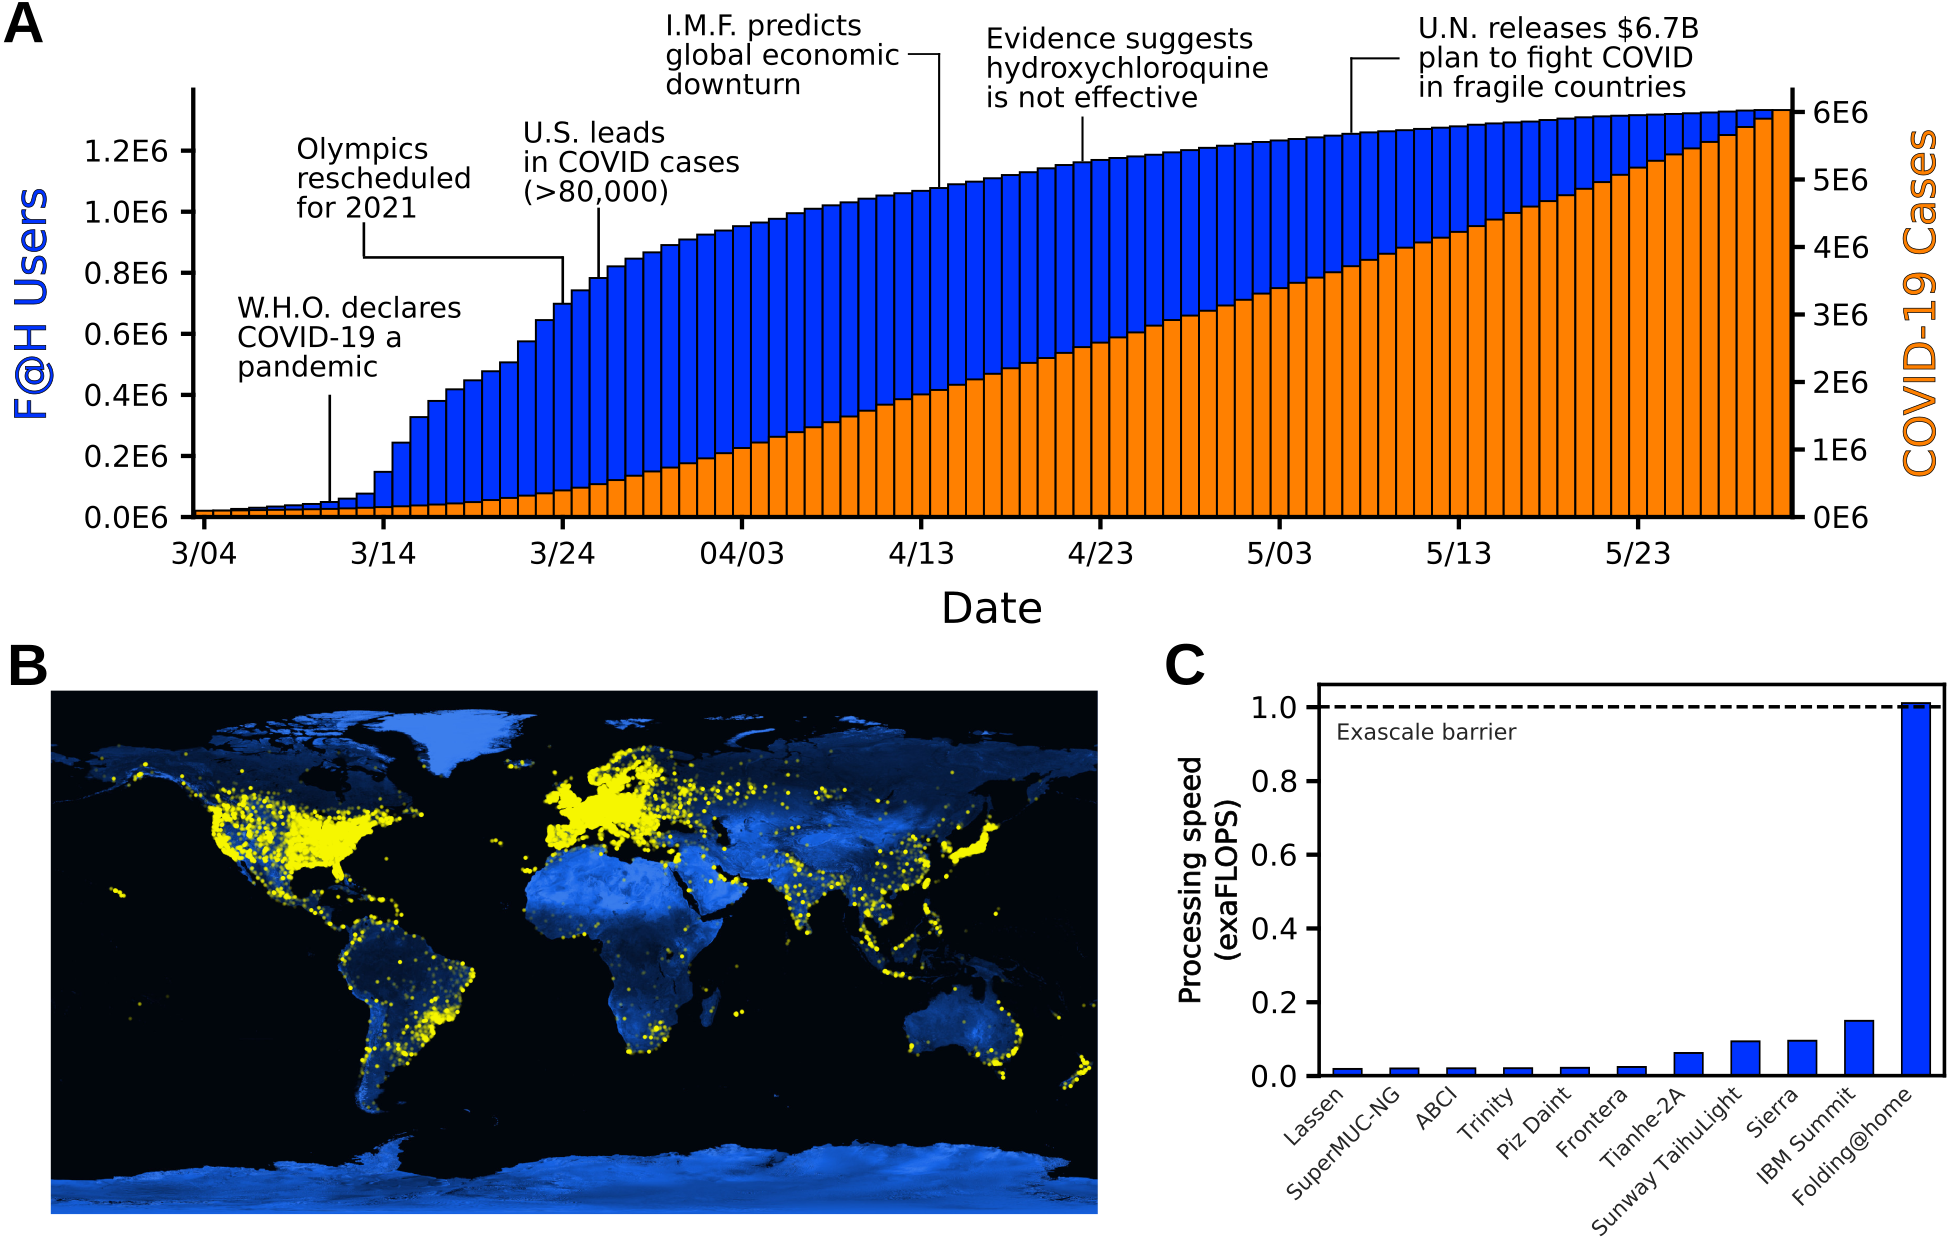
\includegraphics[width=\linewidth]{ch7-fig1.png}
            \caption[Summary of Folding@home’s computational power.]
                {Summary of Folding@home’s computational power. \textbf{A.} The growth and usage of Folding@home in response to COVID-19. Users are colored blue and COVID-19 cases are orange. \textbf{B.} Location of folding at home users. Each yellow dot represents a unique IP address contributing to Folding@home. \textbf{C.} The processing speed of Folding@home and the next 10 fastest supercomputers, in exaFLOPS.}
            \label{fig:ch7-fig1}
        \end{figure}

        Estimating the aggregate compute power of Folding@home is non-trivial due to factors like hardware heterogeneity, measures to maintain volunteers’ anonymity, and the fact that volunteers can turn their machines on and off at-will. Furthermore, volunteers’ machines only communicate with the Folding@home servers at the beginning and end of a work unit, each of which can take anywhere from tens of minutes to a few days depending on the volunteer’s hardware and the protein to simulate. Therefore, we chose to estimate the performance by counting the number of GPUs and CPUs that participated in Folding@home during a three-day window and making a conservative assumption about the computational performance of each device (see Methods for details).

        Given the above, we estimate the peak performance of Folding@home hit 1.01 exaFLOPS. This performance was achieved at a point when ~280,000 GPUs and 4.8 million CPU cores were performing simulations. For reference, that performance is 5-fold greater than the peak performance of the world’s fastest traditional supercomputer, called Summit (Fig. \ref{fig:ch7-fig1}C). It is also more than the top 100 supercomputers combined. Prior to Folding@home, the first exascale supercomputer was not scheduled to come online until the end of 2021.


    \subsection{Unmasking the spike complex}
        The spike complex (S) is a prominent vaccine target that is known to undergo substantial conformational changes as part of its function\cite{kirchdoerfer_stabilized_2018,walls_structure_2020,wrapp_cryo-em_2020}. Structurally, S is composed of three interlocking proteins, with each chain having a cleavage site separating an S1 and S2 fragment. S resides on the virion surface, where it waits to engage with an angiotensin-converting enzyme 2 (ACE2) receptor on a host cell to trigger infection\cite{zhang_angiotensin-converting_2020,hoffmann_sars-cov-2_2020}. The fact that S is exposed on the virion surface makes it an appealing vaccine target. However, it has a number of effective defense strategies. First, S is decorated extensively with glycans that aid in immune evasion by shielding potential antigens\cite{watanabe_vulnerabilities_2020}. S also uses a conformational masking strategy, wherein it predominantly adopts a closed conformation that buries the receptor-binding domains (RBDs) to evade immune surveillance mechanisms. To engage with ACE2, S undergoes rare transitions to an open state that exposes the conserved binding interface of the RBDs. Characterization of the full range of this motion is important for understanding pathogenesis and could provide insights into novel therapeutic options.

        To capture S opening, we employed our goal-oriented adaptive sampling algorithm, FAST, in conjunction with Folding@home. The FAST method iterates between running a batch of simulations, building an MSM, ranking the MSM states based on how likely starting a new simulation from that state is to yield useful data, and starting a new batch of simulations from the top ranked states\cite{zimmerman_fast_2015,zimmerman_how_2016}. The ranking function is designed to balance between favoring structures with a desired geometric feature (in this case opening of S) and broad exploration of conformational space. By balancing exploration-exploitation tradeoffs, FAST often captures conformational changes with orders of magnitude less simulation time than alternative methods. Broadly distributed structures from our FAST simulations were then used as starting points for extensive Folding@home simulations, totaling 1 ms of data, enabling us to obtain a statistically sound final model.

        Our SARS-CoV-2 S protein simulations capture opening of S and substantial conformational heterogeneity in the open state (Fig. \ref{fig:ch7-fig3}). Capturing opening of S is an impressive technical feat given that previous large-scale simulations were unable to observe this essential event for the initiation of infection. Intriguingly, we find that opening occurs only for a single RBD at a time, akin to that observed in cryoEM structures\cite{yuan_cryo-em_2017}. Additionally, we find that the scale of this opening can be substantially larger than has been observed in experimental snapshots (Fig. \ref{fig:ch7-fig3}). The dramatic opening we observe is consistent with the observation that antibodies can bind to regions of the RBD that are deeply buried and seemingly inaccessible in existing experimental snapshots\cite{huo_neutralization_2020}.

        To understand the potential role of conformational masking in determining the lethality and infectivity of different coronaviruses, we also simulated the opening of S proteins from two related viruses: SARS-CoV-1 and HCoV-NL63. These viruses were selected because they also bind the ACE2 receptor but are associated with varying mortality rates. SARS-CoV-1 caused an outbreak in 2003 with a high case fatality rate but has not become a pandemic\cite{zhong_epidemiology_2003}. NL63 was discovered the following year and continues to spread around the globe, although it is significantly less lethal than either SARS virus\cite{van_der_hoek_identification_2004}. We hypothesized that these phenotypic differences may be explained by changes to the S conformational ensemble. Specifically, we propose mutations or other perturbations can increase the S-ACE2 affinity by increasing the probability that S adopts an open conformation or by increasing the affinity between an exposed RBD and ACE2.

        \begin{figure}[!htb] %Positioning code for figure
            \centering
            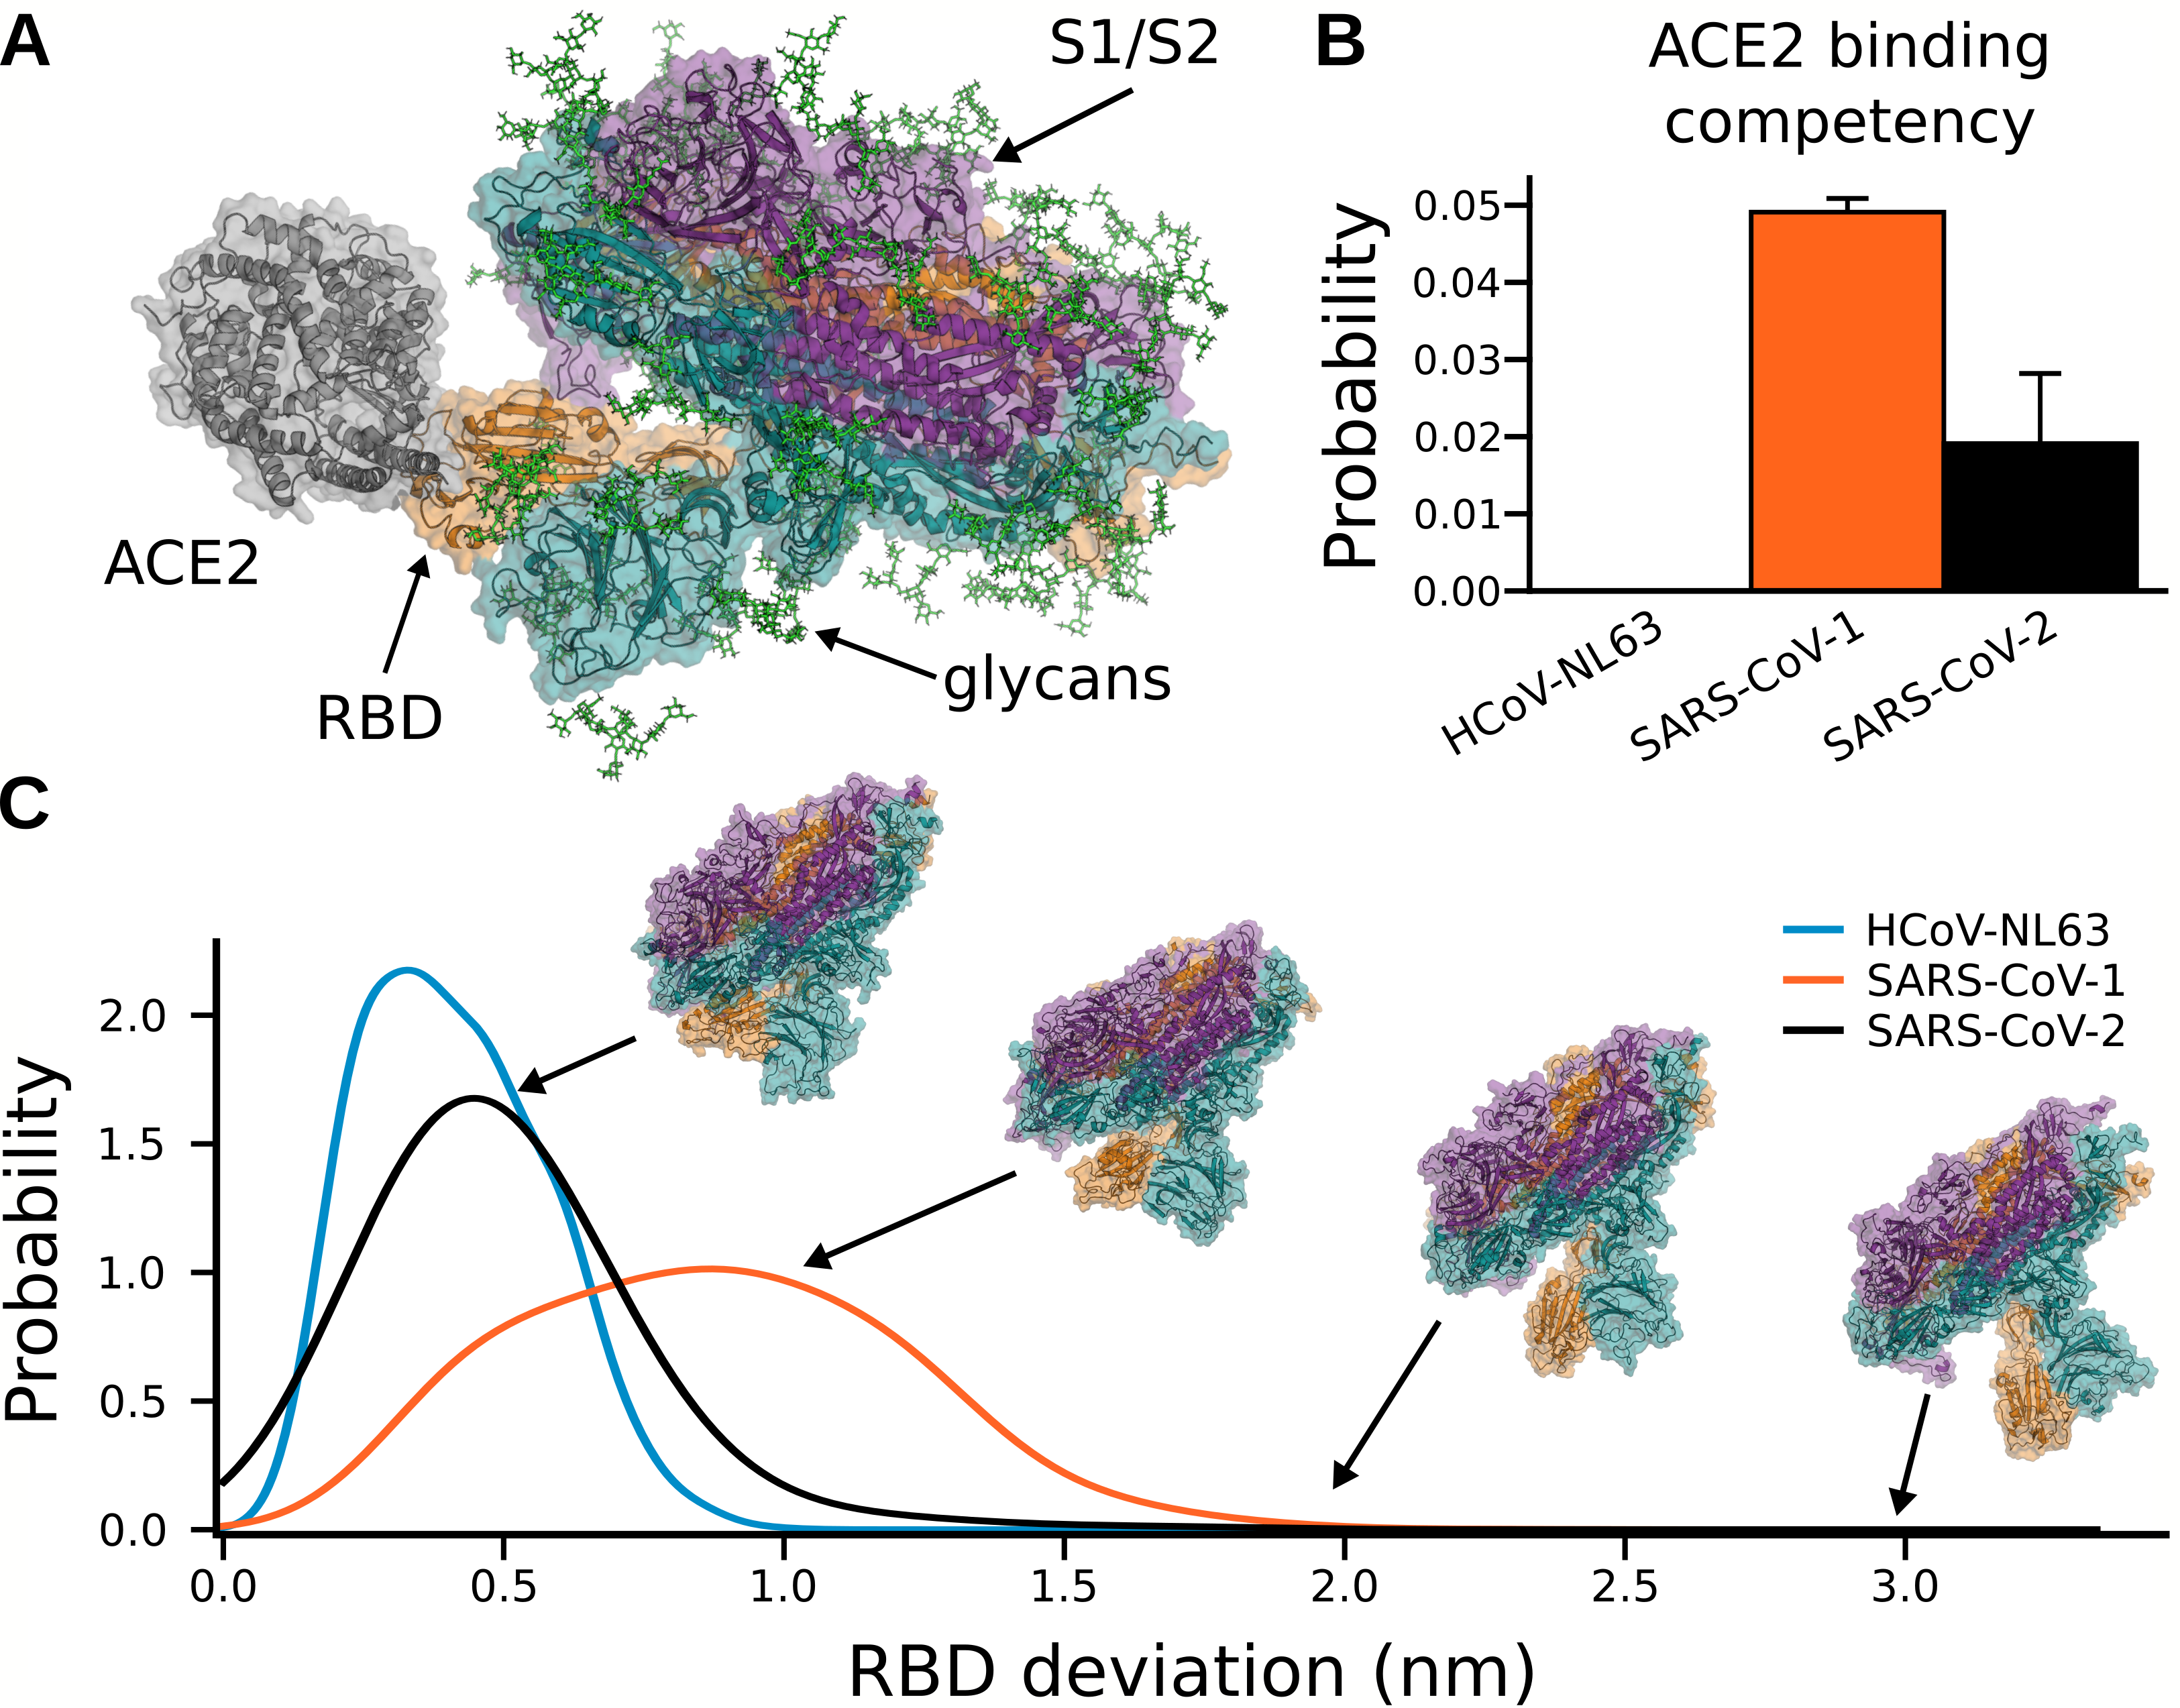
\includegraphics[width=\linewidth]{ch7-fig2.png}
            \caption[Structural characterization of conformational masking in different spike complexes.]
                {Structural characterization of conformational masking in different spike complexes. \textbf{A.} A representative structure of SARS-CoV-2 spike protein in an open conformation, as pulled from our molecular dynamic simulations. ACE2 (gray) is superimposed onto the structure to highlight binding compatibility. The three chains of Spike are illustrated with a cartoon and transparent surface representation (orange, teal, and purple), and glycans are shown as sticks (green). \textbf{B.} The probability that each sequence adopts an ACE2 binding competent pose. HCoV-NL63, SARS-CoV-1, and SARS-CoV-2 are shown as light-blue, orange, and black, respectively. \textbf{C.} The probability that the center of mass of an RBD deviates from its position in the closed state for HCoV-NL63, SARS-CoV-1, and SARS-CoV-2.}
            \label{fig:ch7-fig2}
        \end{figure}

        As expected, the three S complexes have very different propensities to adopt an open state and bind ACE2. Structures from each ensemble were classified as competent to bind ACE2 if superimposing an ACE2-RBD structure on S did not result in any steric clashes between ACE2 and the rest of the S complex. We find that SARS-CoV-1 has the highest population of conformations that can bind to ACE2 without steric clashes, followed by SARS-CoV-2, while opening of NL63 is sufficiently rare that we did not observe ACE2-binding competent conformations in our simulations (Fig. \ref{fig:ch7-fig2}B). Interestingly, S proteins that are more likely to adopt structures that are competent to bind ACE2 are also more likely to adopt highly open structures (Fig. \ref{fig:ch7-fig2}C).

        We also observe a number of interesting correlations between conformational masking, lethality, and infectivity of different coronaviruses. First, more deadly coronaviruses have S proteins with less conformational masking. Second, there is an inverse correlation between S opening and the affinity of an isolated RBD for ACE2 (RBD-ACE2 affinities of ~35 nM, ~44 nM, and ~185 nM for HCoV-NL63, SARS-CoV-2, and SARS-CoV-1, respectively)\cite{wu_crystal_2009,shang_structural_2020}.

        \begin{figure}[!htb] %Positioning code for figure
            \centering
            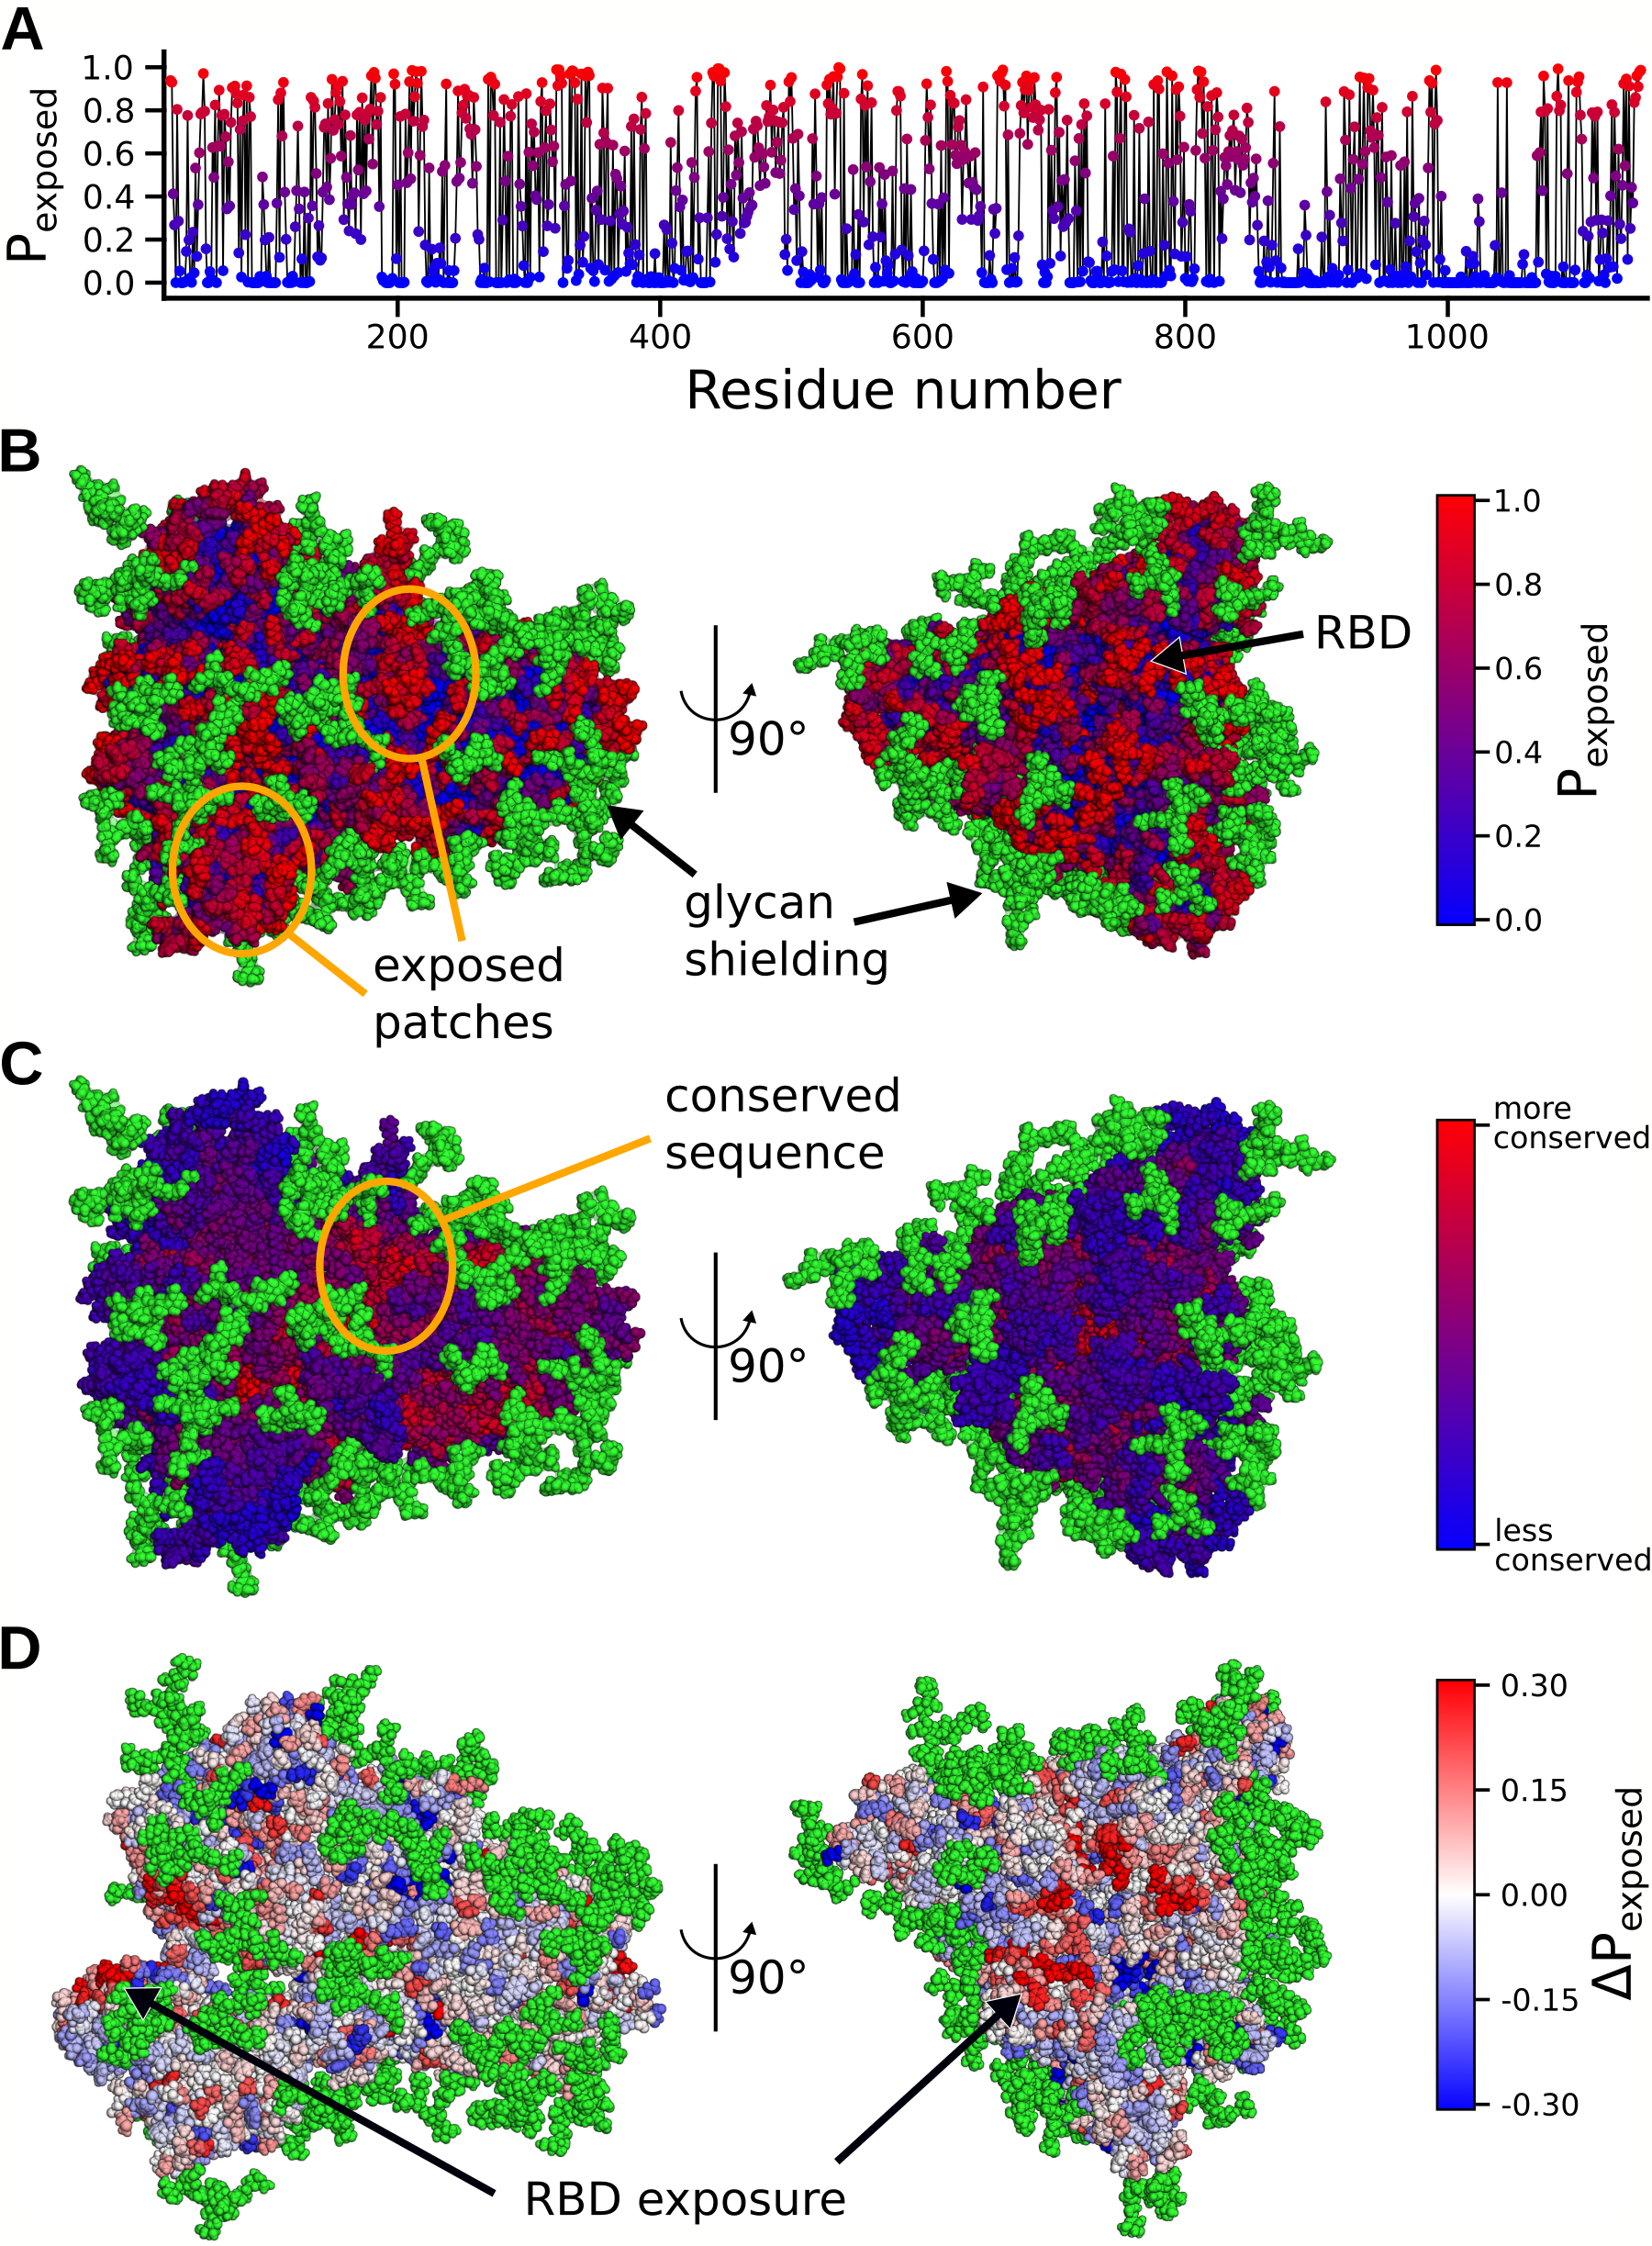
\includegraphics[width=5in]{ch7-fig3.png}
            \caption[Effects of glycan shielding and conformational masking on the accessibility of different parts of the spike to potential therapeutics.]
                {Effects of glycan shielding and conformational masking on the accessibility of different parts of the spike to potential therapeutics. \textbf{A.} The probability that a residue is exposed to potential therapeutics, as determined from our structural ensemble. \textbf{B.} Exposure probabilities colored on the surface of the spike protein. Exposed patches are circled orange. Red residues have a higher probability of being exposed, whereas blue residues have a lower probability of being exposed. \textbf{C.} Sequence conservation score colored onto the Spike protein. A conserved patch on the protein is circled in orange. Red residues have higher conservation, whereas blue residues have lower conservation. \textbf{D.} The difference in the probability that each residue is exposed between the ACE2-binding competent conformations and the entire ensemble. Red residues have a higher probability of being exposed upon opening, whereas blue residues have a lower probability of being exposed.}
            \label{fig:ch7-fig3}
        \end{figure}

        These observations suggest a tradeoff wherein greater conformational masking enables immune evasion but requires a higher affinity between an exposed RBD and ACE2 to successfully infect a host cell. We propose that the NL63 S complex is probably best at evading immune detection but is not as infectious as the SARS viruses because strong conformational masking reduces the overall affinity for ACE2. In contrast, the SARS-CoV-1 S complex adopts open conformations more readily but is also more readily detected by immune surveillance mechanisms. Finally, SARS-CoV-2 balances conformational masking and the RBD-ACE2 affinity in a manner that allows it to evade an immune response while maintaining its ability to infect a host cell. Based on this model, we predict that mutations that increase the probability that the SARS-CoV-2 S complex adopts open conformations may be more lethal but spread less readily.

        Our atomically detailed model of S can enable rapid structure-based vaccine antigen design through identification of regions minimally protected by conformational masking or the glycan shield\cite{graham_structure-based_2019}. To identify these potential epitopes, we calculated the probability that each residue in S could be exposed to therapeutics (e.g. not shielded by a glycan or buried by conformational masking), as shown in Fig. \ref{fig:ch7-fig3}A. Visualizing these values on the protein reveals a few patches of protein surface that are exposed through the glycan shielding (Fig. \ref{fig:ch7-fig3}B). However, another important factor when targeting an antigen is picking a region with a conserved sequence to yield broader and longer lasting efficacy. Not surprisingly, many of the exposed regions do not have a strongly conserved sequence. Promisingly, though, we do find a conserved area with a larger degree of solvent exposure (Fig. \ref{fig:ch7-fig3}C). Another possibility for antigen design is to exploit the opening motion. A number of conserved residues of the RBD show an increase in exposure by \~30\% in ACE2 binding competent structures (Fig. \ref{fig:ch7-fig3}C). Consistent with immunoassays, this region was recently found to be a cluster for neutralizing antibody binding\cite{huo_neutralization_2020,zhong_epidemiology_2003}.


    \subsection{Cryptic pockets and functional dynamics}
        Every protein in SARS-CoV-2 is a potential drug target. So, to understand their role in disease and help progress the design of antivirals, we unleashed the full power of Folding@home to simulate dozens of systems related to pathogenesis. While we are interested in all aspects of a proteins’ functional dynamics, expanding on the number of antiviral targets is of immediate value. Towards this end, we seeded Folding@home simulations from our FAST-pockets adaptive sampling to aid in the discovery of cryptic pockets. We briefly discuss two illustrative examples, out of 36 datasets.
        
        Nonstructural protein number 5 (NSP5, also named the main protease, Mpro, or 3CLpro) is critical for the lifecycle of coronaviruses and is a major target for the design of antivirals\cite{zhang_crystal_2020}. It is highly conserved between coronaviruses, owing to its necessary function of processing polyproteins. NSP5 is only active as a dimer, however it exists in a monomer-dimer equilibrium with estimates of its dissociation constant in the low $\mu$M range\cite{graziano_sars_2006}. Small molecules targeting this protein to inhibit enzymatic activity, either by altering its active site or favoring the inactive monomer state, would be promising broad-spectrum antiviral candidates\cite{goyal_targeting_2020}.

        \begin{figure}[!htb] %Positioning code for figure
            \centering
            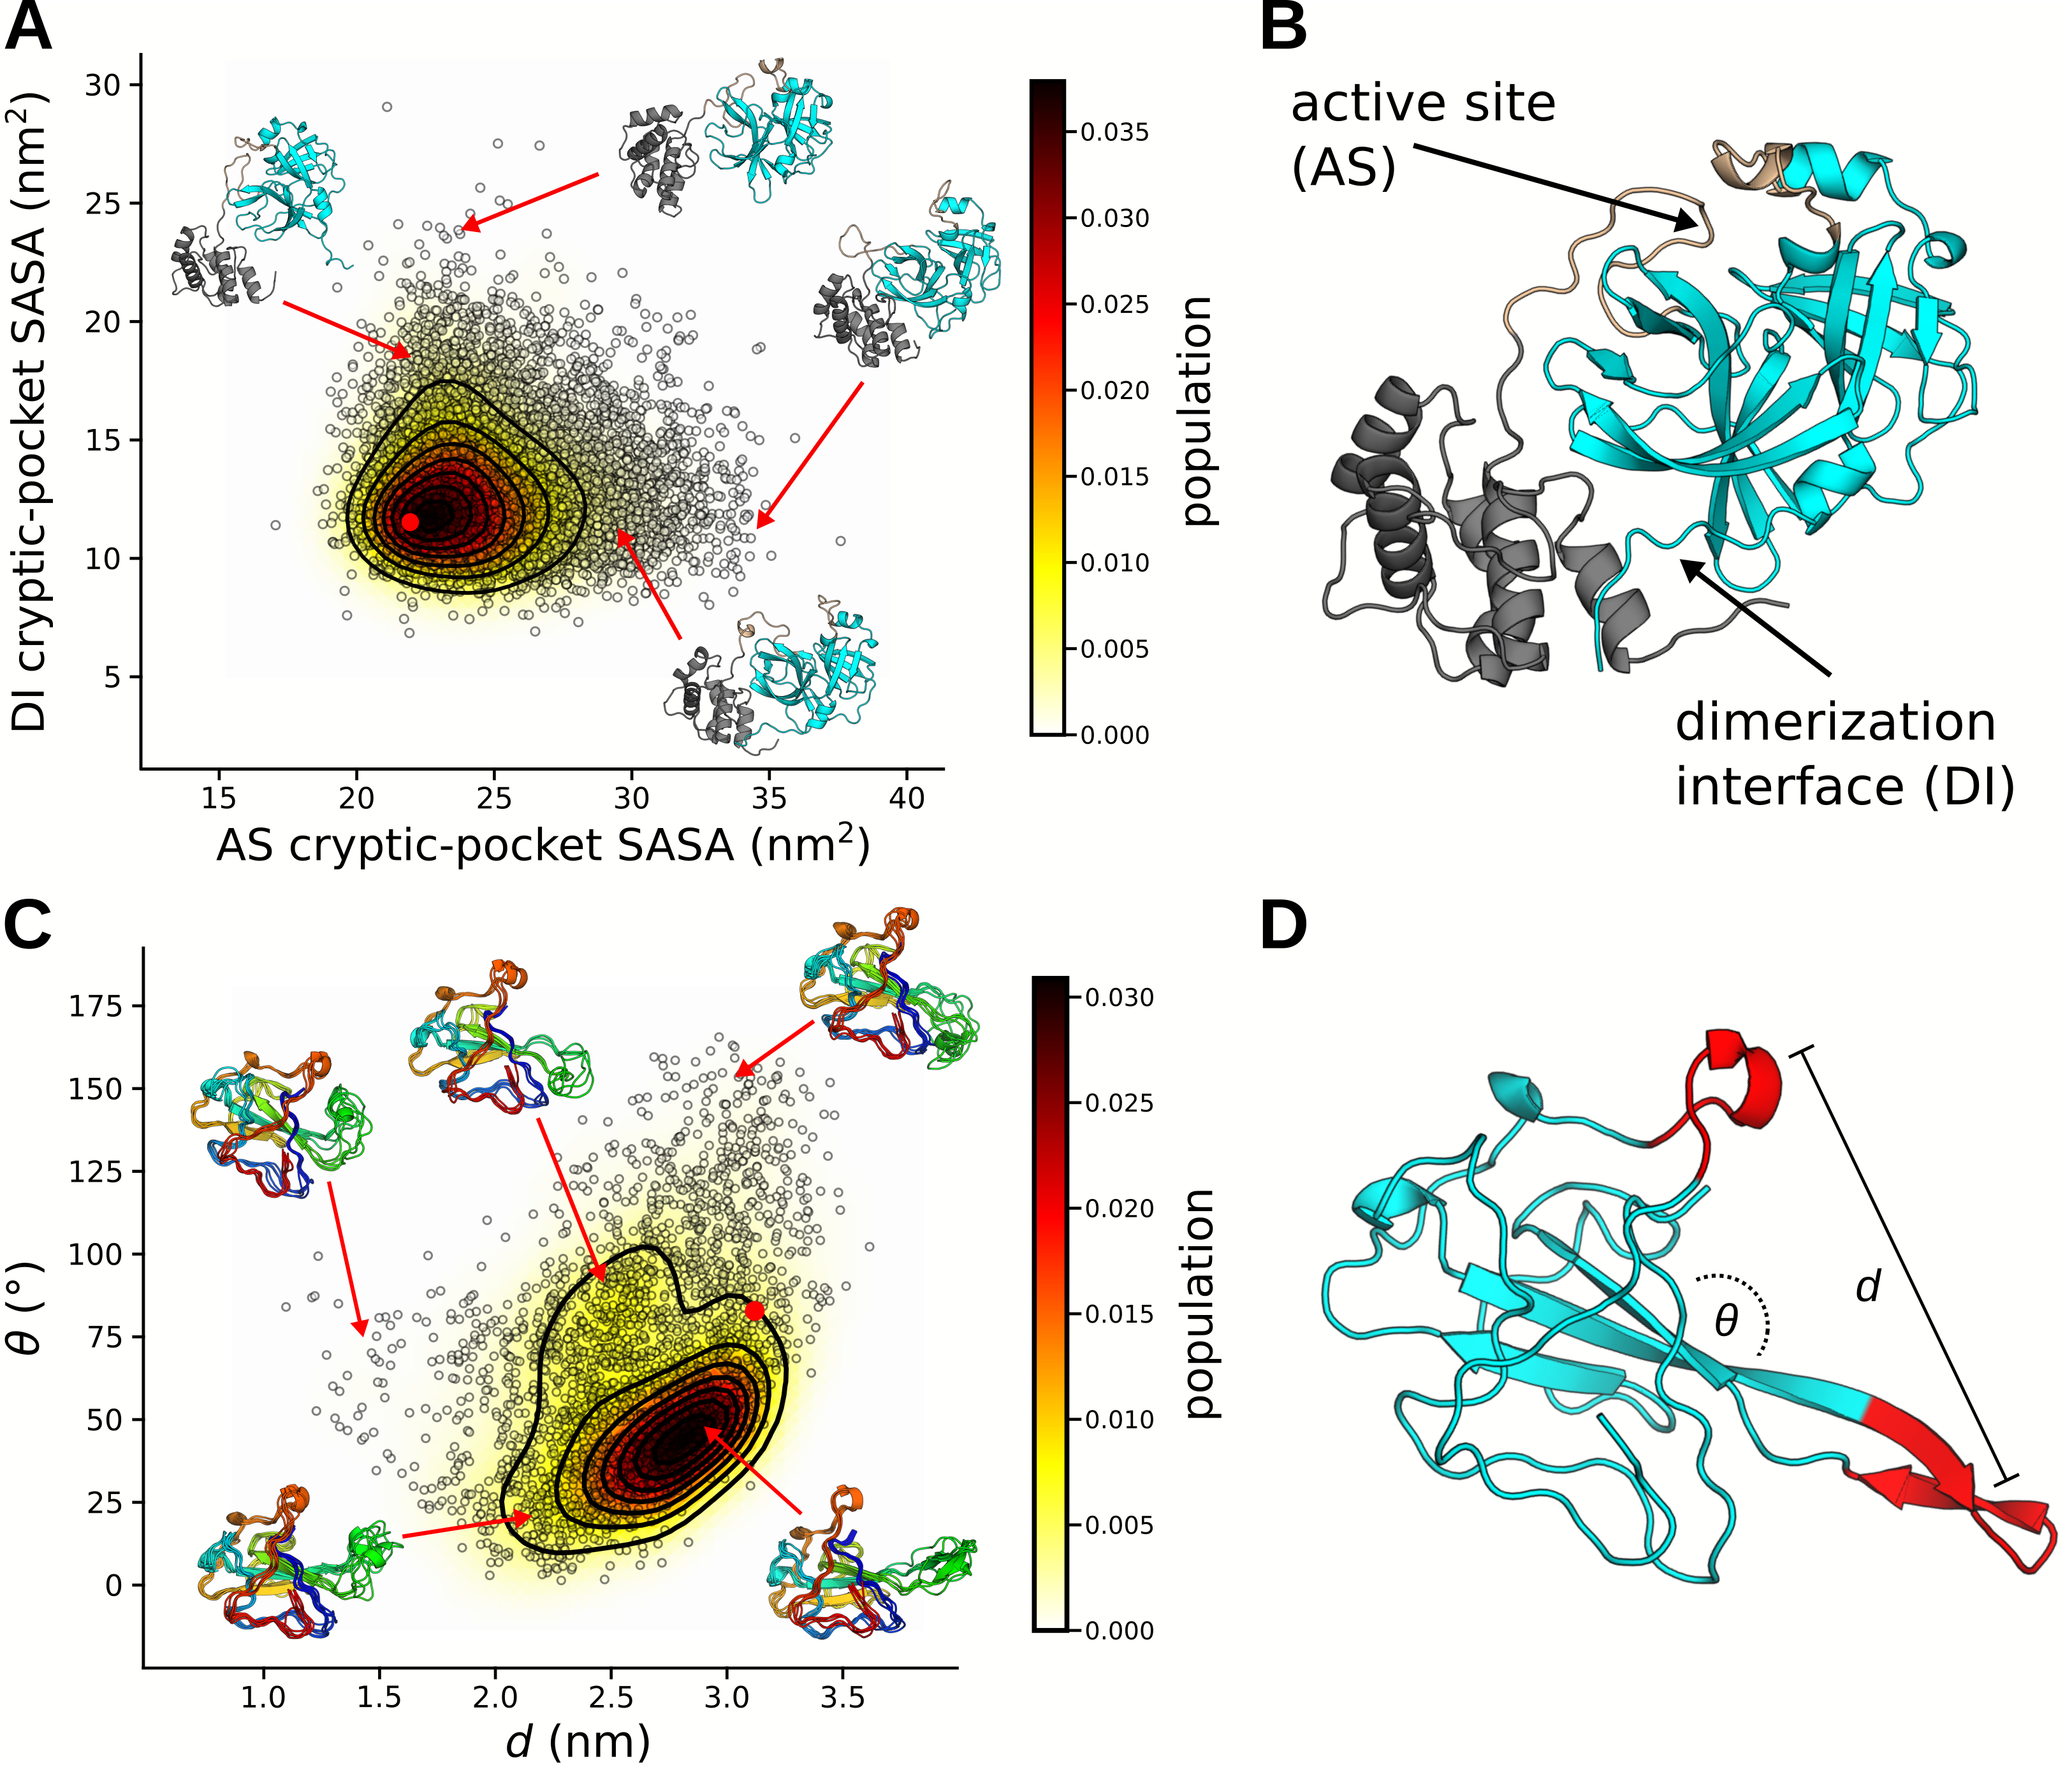
\includegraphics[width=6in]{ch7-fig4.png}
            \caption[Examples of cryptic pockets and functionally-relevant dynamics.]
                {Examples of cryptic pockets and functionally-relevant dynamics. \textbf{A-B)} Conformational ensemble of the main protease (NSP5) projected onto the solvent accessible surface areas (SASAs) of residues surrounding either the active-site or a cryptic pocket. Cluster centers are represented as black circles with representative structures depicted with cartoon. The starting structure for simulations (6Y2E) is shown as a red dot. Domains I and II are colored cyan and domain III is colored gray. The loop of domain III, that covers the active-site residues and is seen to be highly dynamic, is colored tan. \textbf{C-D)} Conformational ensemble of Nucleoprotein projected onto the distance and angle between the positive finger and a nearby loop. Angles were calculated between vectors that point along each red segment in panel D and distances were calculated between their centers of mass. Cluster centers are represented as black circles and representative structures are depicted with cartoon. The starting structure for simulations (6VYO) is shown as a red dot.}
            \label{fig:ch7-fig4}
        \end{figure}

        Our simulations reveal two novel cryptic pockets on NSP5 that expand our current therapeutic options. These are shown in figure \ref{fig:ch7-fig4}A, which projects states from our MSM onto the solvent exposure of residues that make up the pockets. The first cryptic pocket is an expansion of NSP5’s catalytic site. We find that the loop bridging domains II and III is highly dynamic and can fully disengage the protein. This motion may be necessary for catalysis and is similar to motions we have observed previously for the enzyme $\beta$-lactamase\cite{Porter:2019hv}. Owing to its location, a small molecule bound in this pocket is likely to prevent catalysis by obstructing polypeptide association with catalytic residues. The second pocket is a large opening between domains I/II and domain III. Located at the dimerization interface, this pocket offers the possibility to find small molecule or peptide stabilizers that favor the inactive monomer state.

        In addition to cryptic pockets, our data captures many potentially functionally relevant motions within the SARS-CoV-2 proteome. We illustrate this with the SARS-CoV-2 nucleoprotein. The nucleoprotein is a multifunctional protein responsible for major lifecycle events such as viral packaging, transcription, and physically linking RNA to the envelope\cite{mcbride_coronavirus_2014,masters_coronavirus_2019}. As such, we expect the protein to accomplish these goals through a highly dynamic and rich conformational ensemble, akin to context-dependent regulatory modules observed in Ebola virus nucleoprotein\cite{cubuk_sars-cov-2_2020,su_electron_2018}. Investigating the RNA-binding domain, we observe both cryptic pockets and an incredibly dynamic beta-hairpin, which hosts the RNA binding site, referred to as a “positive finger” (Fig. \ref{fig:ch7-fig4}C-D). Our observed conformational heterogeneity of the positive finger is consistent with a structural ensemble determined using solution-state nuclear magnetic resonance spectroscopy\cite{dinesh_structural_2020}. Our simulations also capture numerous states of the putative RNA binding pose, where the positive finger curls up to form a cradle for RNA. These states can provide a structural basis for the design of small molecules that would compete with RNA binding, preventing viral assembly. Additionally, knowledge of these probabilities can provide further insight into the mechanisms and regulation of genome compaction/release.

        The data we present in this paper represents the single largest collection of all-atom simulations. Table \ref{tab:covid-systems-table1} is a comprehensive list of the systems we have simulated. Systems span various oligomerization states, include important complexes, and include representation from multiple coronaviruses. We also include human proteins that are targets for supportive therapies and preventative treatments. To accelerate the discovery of new therapeutics and promote open science, we are posting all of our data online (https://covid.molssi.org/).

        \begin{table}[]
        \centering
        \caption{A list of protein systems we have simulated on Folding@home. Systems are organized by viral strain and include name, oligomerization state, starting structure, number of residues, number of atoms in the system, aggregate simulation time, and the number of cryptic pockets we have identified.\\
        *Missing residues were modeled using Swiss model\cite{waterhouse_swiss-model:_2018}.\\
        **Structural model was generated from a homologous sequence using Swiss model\cite{waterhouse_swiss-model:_2018}.\\
        ***Missing residues were modeled using CHARMM-GUI\cite{cubuk_sars-cov-2_2020,su_electron_2018}}
        \label{tab:covid-systems-table1}
        \resizebox{\textwidth}{!}{\begin{tabular}{|l|l|p{2.5cm}|l|l|l|p{2.5cm}|}
                \hline
                System name &
                  Oligomerization &
                  Initial structure (homology) &
                  Residues &
                  Atoms in system &
                  Aggregate simulation time (us) &
                  Cryptic pockets discovered \\ \hline
                                                  &                &         &      &        &        &     \\ \hline
                \textbf{SARS-CoV-2}               &                &         &      &        &        &     \\ \hline
                NSP3 (Macrodomain ÒXÓ)            & Monomer        & 6W02    & 167  & 23907  & 10,531 & TBD \\ \hline
                NSP3 (Papain-like protease 2, PL2pro) &
                  Monomer &
                  3E9S** &
                  306 &
                  97285 &
                  621 &
                  TBD \\ \hline
                NSP5 (main protease, 3CLpro)      & Monomer        & 6Y2E    & 306  & 64791  & 6,050  & TBD \\ \hline
                NSP5 (main protease, 3CLpro)      & Dimer          & 6Y2E    & 612  & 77331  & 2,189  & TBD \\ \hline
                NSP7                              & Monomer        & 5F22**  & 79   & 20094  & 7,622  & TBD \\ \hline
                NSP8                              & Monomer        & 2AHM**  & 191  & 156282 & 1,259  & TBD \\ \hline
                NSP9                              & Dimer          & 6W4B*   & 226  & 49885  & 7,503  & TBD \\ \hline
                NSP10                             & Monomer        & 6W4H*   & 131  & 29560  & 3,050  & TBD \\ \hline
                NSP12 (polymerase)                & Monomer        & 6NUR**  & 891  & 186622 & 1,114  & TBD \\ \hline
                NSP13 (helicase)                  & Monomer        & 6JYT**  & 596  & 129368 & 939    & TBD \\ \hline
                NSP14                             & Monomer        & 5C8S**  & 527  & 216380 & 359    & TBD \\ \hline
                NSP15                             & Monomer        & 6VWW    & 347  & 67345  & 3,618  & TBD \\ \hline
                NSP15                             & Hexamer        & 6VWW    & 2082 & 230339 & 1,461  & TBD \\ \hline
                NSP16                             & Monomer        & 6W4H*   & 298  & 45672  & 2,684  & TBD \\ \hline
                Nucleoprotein (RBD)               & Monomer        & 6VYO    & 173  & 29125  & 8,742  & TBD \\ \hline
                Nucleoprotein Dimerization Domain & Monomer        & 6YUN*   & 118  & 34905  & 2,420  & TBD \\ \hline
                Nucleoprotein Dimerization Domain & Dimer          & 6YUN*   & 236  & 72733  & 1,251  & TBD \\ \hline
                Spike                             & Trimer         & 6VXX*** & 3363 & 442881 & 949    & TBD \\ \hline
                NSP7 / NSP8 / NSP12               & Trimer complex & 6NUR**  & 1184 & 215694 & 291    & TBD \\ \hline
                NSP10 / NSP14                     & Dimer complex  & 5C8S**  & 688  & 226672 & 469    & TBD \\ \hline
                NSP10 / NSP16                     & Dimer complex  & 6W4H*   & 429  & 63752  & 2,415  & TBD \\ \hline
                                                  &                &         &      &        &        &     \\ \hline
                \textbf{SARS-CoV-1}               &                &         &      &        &        &     \\ \hline
                NSP3 (Macrodomain ÒXÓ)            & Monomer        & 2FAV    & 172  & 33117  & 507    & TBD \\ \hline
                NSP9                              & Dimer          & 1QZ8*   & 226  & 49599  & 6,736  & TBD \\ \hline
                NSP15                             & Monomer        & 2H85    & 345  & 67345  & 2,663  & TBD \\ \hline
                NSP15                             & Hexamer        & 2H85    & 2070 & 230339 & 829    & TBD \\ \hline
                Nucleoprotein RBD                 & Monomer        & 2OFZ    & 174  & 29125  & 4,124  & TBD \\ \hline
                Nucleoprotein Dimerization Domain & Monomer        & 2GIB    & 370  & 34905  & 874    & TBD \\ \hline
                Nucleoprotein Dimerization Domain & Dimer          & 2GIB    & 740  & 72733  & 427    & TBD \\ \hline
                Spike                             & Trimer         & 5X58*** & 3261 & 375851 & 784    & TBD \\ \hline
                NSP10 / NSP16                     & Dimer complex  & 6W4H**  & 425  & 69589  & 175    & TBD \\ \hline
                                                  &                &         &      &        &        &     \\ \hline
                \textbf{Human}                    &                &         &      &        &        &     \\ \hline
                IL6                               & Monomer        & 1ALU    & 166  & 26855  & 1,263  & TBD \\ \hline
                IL6-R                             & Monomer        & 1N26    & 299  & 149764 & 132    & TBD \\ \hline
                ACE2                              & Monomer        & 6LZG    & 596  & 75787  & 244    & TBD \\ \hline
                                                  &                &         &      &        &        &     \\ \hline
                \textbf{MERS}                     &                &         &      &        &        &     \\ \hline
                NSP13                             & Monomer        & 5WWP    & 596  & 121134 & 288    & TBD \\ \hline
                NSP10 / NSP16                     & Dimer Complex  & 6W4H**  & 424  & 69127  & 174    & TBD \\ \hline
                                                  &                &         &      &        &        &     \\ \hline
                \textbf{HCoV-NL63}                &                &         &      &        &        &     \\ \hline
                Spike                             & Trimer         & 5SZS*** & 3606 & 453348 & 618    & TBD \\ \hline
                \end{tabular}}
        \end{table}

    \section{Discussion}
        In this work, we have utilized the largest computer in the world to tackle a global threat. The pandemic caused by SARS-CoV-2 has necessitated a call-to-arms; a call that over a million citizen-scientists have answered, generating more than 0.1 seconds of simulation data. The unprecedented scale of these simulations has helped to characterize crucial stages of infection. We find that spike proteins have a strong trade-off between making ACE2 binding interfaces accessible to infiltrate cells and conformationally masking epitopes to subvert immune responses. SARS-CoV-2 represents a more optimal tradeoff than related coronaviruses, which may explain its success in spreading globally. Our simulations also provide an atomically detailed roadmap for targeting proteins for vaccines and antivirals. Furthermore, we are working on making a comprehensive repository of cryptic pockets hosted online to accelerate the development of novel therapeutics.
    
        Beyond SARS-CoV-2, we expect this work to aid in a better understanding of the roles of proteins in the coronaviridae family. Coronaviruses have been around for millennia, yet many of their proteins are still poorly understood. Because climate change has made zoonotic transmission events more commonplace, it is imperative that we continue to perform basic research on these viruses to better protect us from future pandemics. For each protein system in Table \ref{tab:covid-systems-table1}, an extraordinary amount of sampling has led to the generation of a quantitative map of its conformational landscape. There is still much to learn about coronavirus function and these conformational ensembles contain a wealth of information to pull from.
    
        While we have aggressively targeted research on SARS-CoV-2, Folding@home is a general platform for running molecular dynamics simulations at scale. Before the COVID-19 pandemic, Folding@home was already generating datasets that were orders of magnitude greater than from conventional means. With our explosive growth, our compute power has increased around 100-fold. Our work here highlights the incredible utility this compute power has to rapidly understand health, disease, and aid in drug design. Both in terms of scale and approach, we are in a new frontier of using molecular dynamics simulations to understand biophysics; the complex task of simulating an organism’s entire proteome could become commonplace. With the continued support of the citizen scientists that have made this work possible, we have the opportunity to make a profound impact on other global health crises such as cancer, neurodegenerative diseases, and antibiotic resistance.

    \section{Methods}
    \subsection{System preparations}
        All simulations were prepared using Gromacs 2020\cite{Abraham:2015gj}. Initial structures were placed in a dodecahedron box that extends 1.0 nm beyond the protein in any dimension. Systems were then solvated and energy minimized with a steepest descents algorithm until the maximum force fell below 100 kJ/mol/nm using a step size of 0.01 nm and a cutoff distance of 1.2 nm for the neighbor list, Coulomb interactions, and van der Waals interactions. The AMBER03 force field was used for all systems except spike protein with glycans, which used CHARMM36\cite{Duan:2003gt,huang_charmm36_2013}. All simulations were simulated with explicit TIP3P solvent\cite{Jorgensen:1983fl}.
        
        Systems were then equilibrated for 1.0 ns, where all bonds were constrained with the LINCS algorithm and virtual sites were used to allow a 4 fs time step\cite{Feenstra:1999ue,Hess:2008fl}. Cutoffs of 1.1 nm were used for the neighbor list with 0.9 for Coulomb and van der Waals interactions. The Verlet cutoff scheme was used for the neighbor list. The stochastic velocity rescaling (v-rescale) thermostat was used to hold the temperature at 300 K\cite{Bussi:2007cs}.

    \subsection{Adaptive sampling simulations}
        The FAST algorithm was employed for each protein in Table \ref{tab:covid-systems-table1} to enhance conformational sampling and quickly explore dominant motions. The procedure for FAST simulations is as follows: 1) run initial simulations, 2) build MSM, 3) rank states based on FAST ranking, 4) restart simulations from the top ranked states, 5) repeat steps 2-4 until ranking is optimized. For each system, MSMs were generated after each round of sampling using a k-centers clustering algorithm based on the RMSD between select atoms. Clustering continued until the maximum distance of a frame to a cluster center fell within a predefined cutoff. In addition to the FAST ranking, a similarity penalty was added to promote conformational diversity in starting structures, as has been described previously\cite{zimmerman_prediction_2017}.

        FAST-distance simulations of all Spike proteins were run at 310 K on the Microsoft Azure cloud computing platform. The FAST-distance ranking favored states with greater RBD openings using a set of distances between atoms. Each round of sampling was performed with 22 independent simulations that were 40 ns in length (0.88 $\mu$s aggregate sampling per round), where the number of rounds totaled 13 (11.44 $\mu$s), 22 (19.36 $\mu$s), and 17 (14.96 $\mu$s), for SARS-CoV-1, SARS-CoV-2, and HCoV-NL63, respectively.

        For all other proteins, FAST-pocket simulations were run at 300 K for 6 rounds, with 10 simulations per round, where each simulation was 40 ns in length (2.4 $\mu$s aggregate simulation). The FAST-pocket ranking function favored restarting simulations from states with large pocket openings. Pocket volumes were calculated using the LIGSITE algorithm\cite{hendlich_ligsite:_1997}.

    \subsection{Folding@home simulations}
        For each adaptive sampling run, a conformationally diverse set of structures was selected to be run on Folding@home. Structures came from the final k-centers clustering of adaptive sampling, as is described above. Simulations were deployed using a simulation core based on either GROMACS 5.0.4 or OpenMM 7.4.1 \cite{Abraham:2015gj,eastman_openmm_2017}.


    \subsection{Markov state models}
        A Markov state model is a network representation of a free energy landscape and is a key tool for making sense of molecular dynamics simulations\cite{Husic:2018iz}. All MSMs were built using our python package, enspara\cite{porter2018enspara}. Each system was clustered with the combined FAST and Folding@home datasets. In the case of spike proteins, states were defined geometrically based on the RMSD between backbone C$\alpha$ coordinates. States were generated as the top 3000 centers from a k-centers clustering algorithm. All other proteins were clustered based on the euclidean distance between the solvent accessible surface area of residues, as is described previously\cite{Porter:2019hv}. Systems generated either 2500, 5000, 7500, or 10000 cluster centers from a k-centers clustering algorithm. Select systems were refined with 1-10 k-medoid sweeps. Transition probability matrices were produced by counting transitions between states, adding a prior count of $1/n_states$, and row-normalizing, as is described previously\cite{Zimmerman:2018jn}. Equilibrium populations were calculated as the eigenvector of the transition probability matrix with an eigenvalue of one.

    \subsection{Spike/ACE2 binding competency}
        To determine Spike protein binding competency to ACE2 the following structures of the RBD bound to ACE2 were used: 3D0G, 6M0J, and 3KBH, for SARS-CoV-1, SARS-CoV-2, and HCoV-NL63, respectively. The RBD of the bound complex was superimposed onto each RBD for structures in our MSM. Steric clashes were then determined between backbone atoms on the ACE2 molecule and the rest of the spike protein. If any of the structures had a superposition that resulted in no clashes, it was deemed binding competent.


    \subsection{Cryptic pockets and solvent accessible surface area}
        For ease of detecting cryptic pockets and other functional motions, we employed our exposon analysis method\cite{Porter:2019hv}. This method correlates the solvent exposure between residues to find concerted motions that tend to represent cryptic pocket openings. Solvent accessible surface area calculations were computed using the Shrake-Rupley algorithm as implemented in the python package MDTraj\cite{McGibbon:2015fv}. For all proteins and complexes, a solvent probe radius of 0.28 nm was used, which has been shown to produce a reasonable clustering and exposon map\cite{Porter:2019hv}.

        Spike protein solvent accessible surface areas for SARS-CoV-2 were computed with glycan chains modeled onto each cluster center. Multiple glycan rotamers were sampled for each state and accessible surface areas for each residue were weighted based on MSM equilibrium populations.

    \subsection{Sequence conservation}
        Sequence conservation of spike proteins was calculated using the Uniprot database\cite{the_uniprot_consortium_uniprot:_2019}. Sequences between 30\% - 90\% were pulled and aligned with the Muscle algorithm\cite{edgar_muscle:_2004}. The entropy at each position was calculated to quantify variability of amino acids. Conservation was defined as one minus the entropy\cite{Shannon:1948iy}.

    \section{Acknowledgements}
        We are extremely grateful to all the citizen scientists who contributed their compute power to make this work possible, and members of the Folding@home community who volunteered to help with everything from technical support to translating content into multiple languages. Thanks to Microsoft AI for Health for helping us use Azure to run adaptive sampling simulations, and to UKRI for providing compute resources to parallelize data analysis. Thanks to Pure Storage for providing a FlashBlade system to store our large datasets, to Seagate and Micron for additional storage, and to MolSSI for helping organize public datasets. Thanks to Avast, AWS, Cisco, Linus Tech Tips, Microsoft Azure, Oracle, and VMware for helping us to scale-up Folding@home’s server-side infrastructure to keep up with the tremendous growth we experienced in such a short time. Thanks to AMD, ARM and Neocortix, and Intel for helping to improve the performance of Folding@home on their hardware. Thanks to all of the above companies for spreading the word about Folding@home, and also to A16Z, Best Buy, CCP, CoreWeave, Daimler Truck AG, Dell, GitHub, HP, La Liga, Media Monks, Microcenter, NVIDIA, and Telefonica. Thanks to CERN and the particle physics community for providing guidance on data management strategies and to DataDog for server monitoring services. GRB and his lab were supported by funding from Avast, the Center for the Science and Engineering of Living Systems (CSELS), an NSF RAPID award, NSF CAREER Award MCB-1552471, NIH R01 GM124007, a Burroughs Wellcome Fund Career Award at the Scientific Interface, and a Packard Fellowship for Science and Engineering. JDC acknowledges support from NIH grant P30 CA008748 and NIH grant R01 GM121505. VAV and MFDH acknowledge support from NIH grant R01 GM123296.

    \section{Disclosures}
        JDC is a current member of the Scientific Advisory Board of OpenEye Scientific Software and a consultant to Foresite Laboratories. The Chodera laboratory receives or has received funding from multiple sources, including the National Institutes of Health, the National Science Foundation, the Parker Institute for Cancer Immunotherapy, Relay Therapeutics, Entasis Therapeutics, Silicon Therapeutics, EMD Serono (Merck KGaA), AstraZeneca, Vir Biotechnology, Bayer, XtalPi, the Molecular Sciences Software Institute, the Starr Cancer Consortium, the Open Force Field Consortium, Cycle for Survival, a Louis V. Gerstner Young Investigator Award, and the Sloan Kettering Institute. A complete funding history for the Chodera lab can be found at http://choderalab.org/funding.

    
    % \section{Supplemental material}
    %     \renewcommand{\thefigure}{\arabic{chapter}.S\arabic{figure}}
    %     \setcounter{figure}{0}
        %Chapter 2 supplemental figures get labeled as Figure 2.S1 - 2.S(N). These still automatically pull into the List of Figures. You can do something similar for supplemental tables.
% \bibliography{../References}
% \bibliographystyle{unsrt}

\end{document}